
% JJ

%%%%%%%%%
%
% Subsection: Timing Testing
%
%%%%%%%%%

\subsection{Timing Testing}

The timing data collected does not provide a clear understanding of the scalability of the algorithms. Figure~\ref{fig:plane} displays the performance data collected for varying values of nodes and data rows. The height of the chart represents the time to execute the program. The x-axis is \texttt{log(TotalLines)}, the z-axis is the number of nodes the program was executed on, and the y-axis is the \texttt{log(Runtime)}.


\begin{figure}
\centering
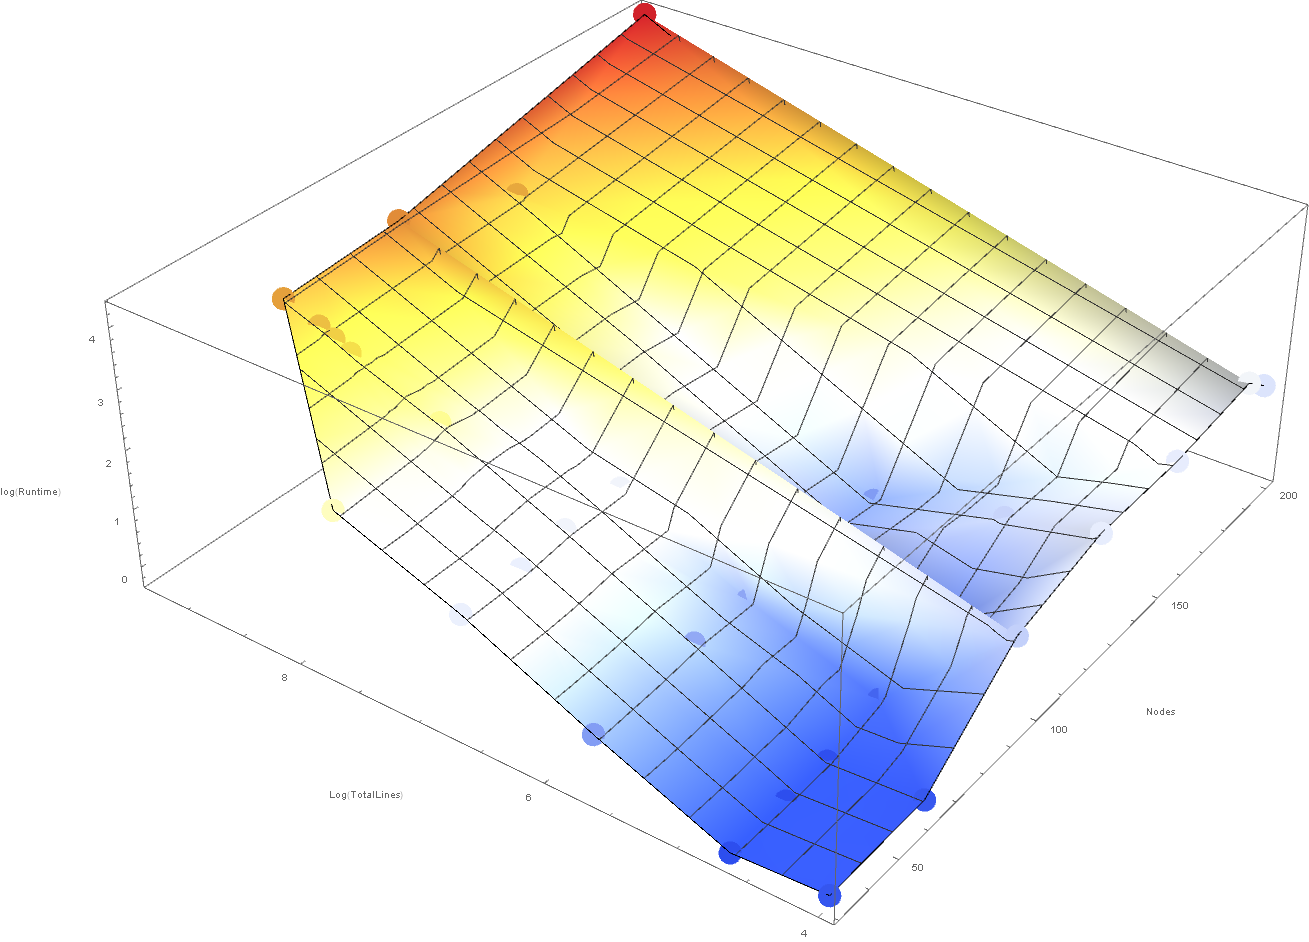
\includegraphics[width=0.7\textwidth]{./images/runtimes.png}
\caption{Execution time versus nodes and total lines}
\label{fig:plane}
\end{figure}


The upper left of the plane is truncated due to the inability to execute the program for large datasets on fewer nodes. 20\% of the timing data had to be excluded due to varying multiple parameters simultaneously. The original plan had been to perform a fully-nested Analysis of Variance (ANOVA) test on the data to understand which parameters impacted performanced the greatest. However, due to the programming challenges encountered and cluster utilization, this did not occur. Another cause of the irregular performance is the sharing of the cluster. Teams would run tests using \texttt{qlogin} (including Team Metropolis) rather than submitting them through \texttt{qsub} to allow the job scheduler.

A subset of the performance data is presented in the following table.

\begin{tabular}{r r r r r}
 & \multicolumn{4}{c}{\textbf{Execution times (seconds)}} \\
\textbf{Total Lines} & \underline{32 Cores} & \underline{64 Cores} & \underline{128 Cores} & \underline{200 Cores} \\
       50,000 &   0.55 &     0.57 &     15.49 & 15.45 \\
      500,000 &   4.18 &     5.51 &      4.06 & 9.18 \\
   5,000,0000 &  39.49 &    50.01 &           & 65.05 \\
   50,000,000 & 234.73 &   404.49 &           & 574.71 \\
  500,000,000 &        & 2,094.11 &  3,685.35 & \\
1,000,000,000 &        & 4,146.69 &           &  \\
2,000,000,000 &        &          &           & 21,355.30 \\ 
\end{tabular}

The execution time of the program increases as more nodes are added while keeping the total data rows constant. One possible explanation for this is that on smaller numbers of nodes the job was not running on systems occupied by other teams. However, as the number of nodes increased, the job began contending for resources with other jobs.

\begin{figure}
\centering
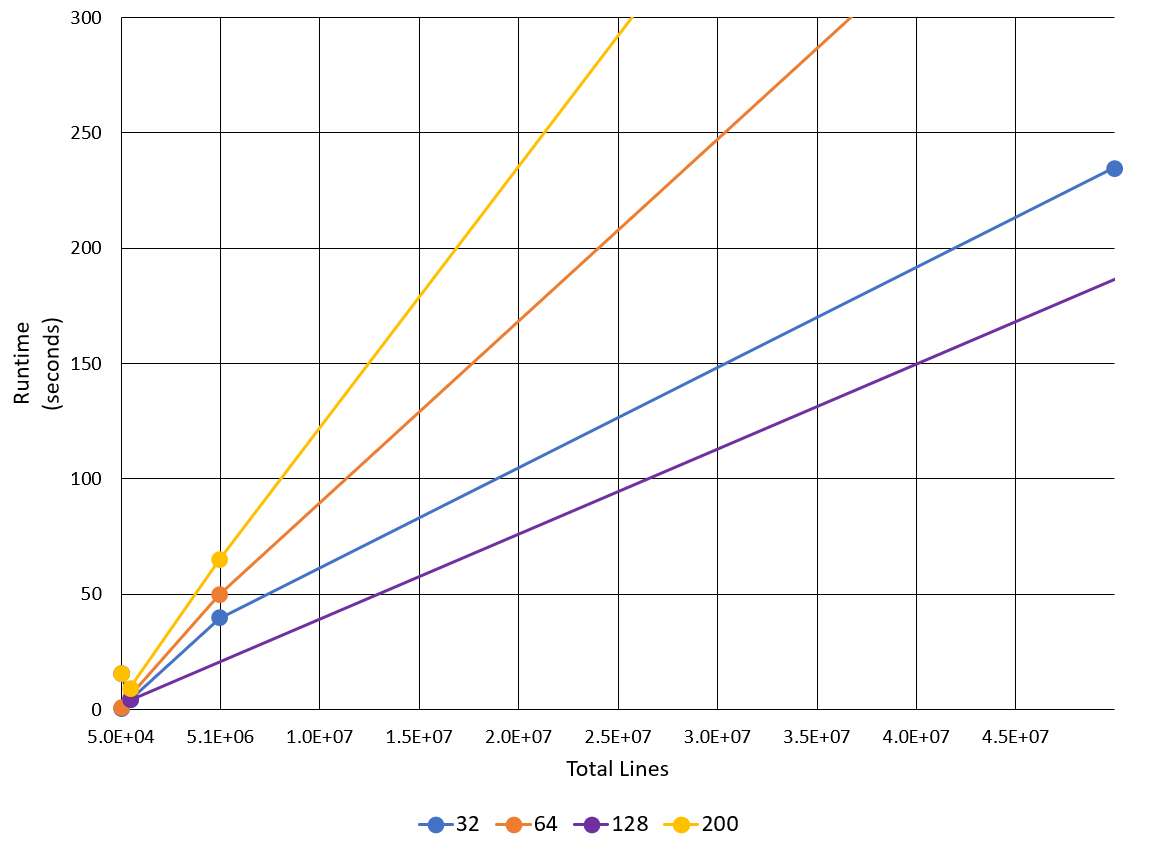
\includegraphics[width=0.7\textwidth]{./images/Runtime1.png}
\caption{Execution time versus nodes for total lines from 50,000 to 50,000,000}
\label{fig:lownums}
\end{figure}

\begin{figure}
\centering
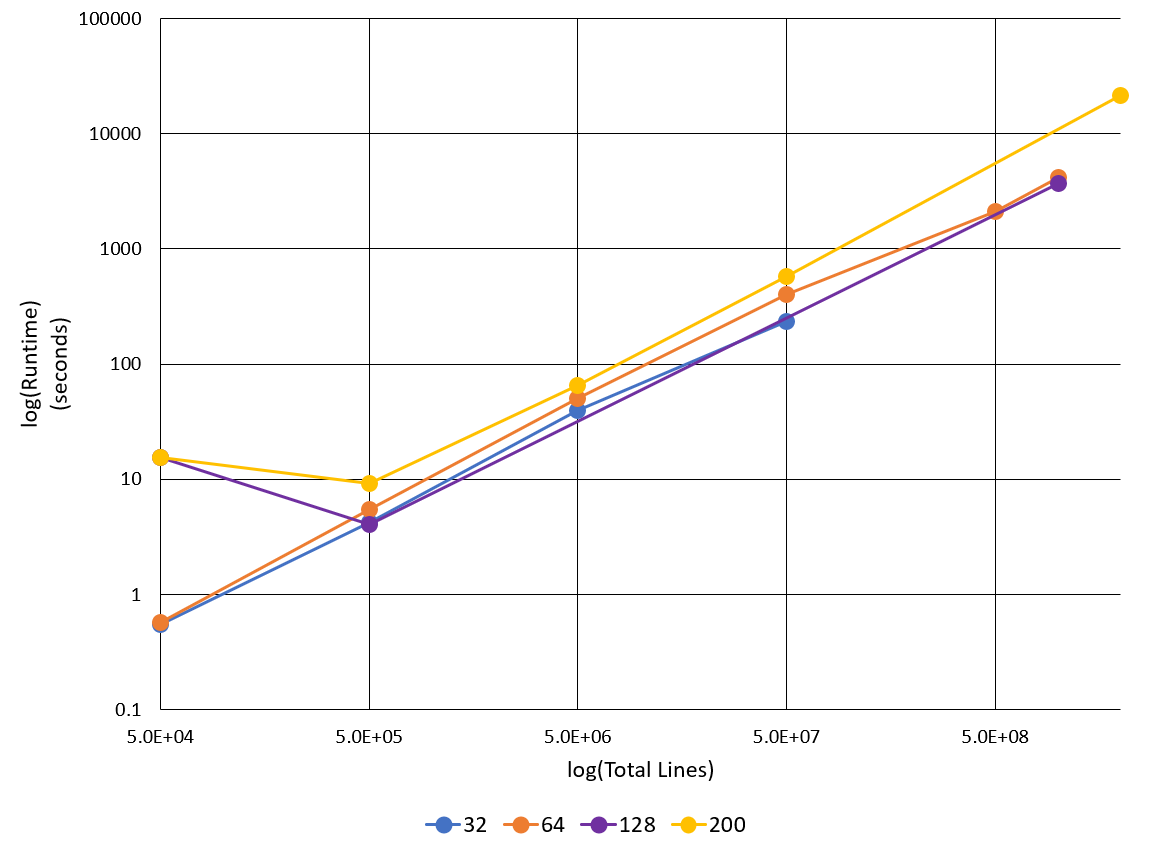
\includegraphics[width=0.7\textwidth]{./images/Runtime2.png}
\caption{Execution time versus nodes and total lines from 50,000 to 2,000,000,000}
\label{fig:allnums}
\end{figure}

Figure~\ref{fig:lownums} shows the runtimes for four different job sizes (32, 64, 128, and 200 nodes) with varying numbers of data rows from 50,000 to 50,000,000. Figure~\ref{fig:allnums} shows the runtimes from 50,000 to 2,000,000,000 (the largest job size that completed successfully).


\begin{figure}
\centering
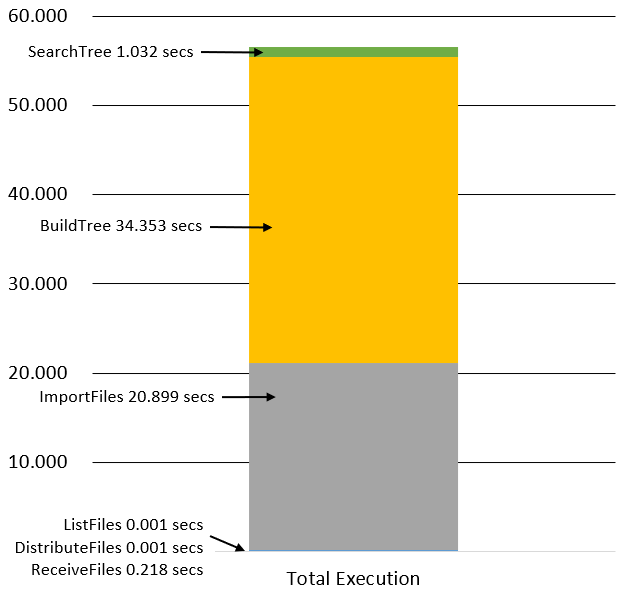
\includegraphics[width=0.7\textwidth]{./images/Runtime3.png}
\caption{Execution time by function for 5,000,000 total lines and 1,000 search rows}
\label{fig:breakdown}
\end{figure}


Figure~\ref{fig:breakdown} provides a glimpse into the performance of the various functions of the program, and the results are provided in the following table.

\begin{tabular}{l r r l}
\textbf{Function}         & \textbf{Runtime}        & \textbf{Percent} & \textbf{Note} \\
ListFiles        &  0.001 seconds & 0.002\% & Lists contents of data directory \\
DistributeFiles  &  0.001 seconds & 0.002\% & Distributes filenames round-robin \\
& & & to nodes \\
ReceiveFiles     &  0.218 seconds & 0.386\% & Receives list of files to process \\
ImportFiles      & 20.889 seconds & 36.976\% & Reads assigned text files into memory \\
BuildTree        & 34.353 seconds & 60.808\% & Builds parallel and serial trees. Includes \\
& & & data swapping among nodes.\\
SearchTree       &  1.032 seconds & 1.827\% & Searches the constructed tree and \\
& & &  produces results \\
\textbf{Total}   & \textbf{56.494 seconds} & \textbf{100.000\%} & \\
\end{tabular}


These results were not unexpected.


%%%%%%%%%
%
% Subsection: Search Results
%
%%%%%%%%%

\subsection{Search Results}

The program exports a table at the end of the run displaying the number of points contained in each of three radii centered at each row of points from  \texttt{datafile00501.txt}. The first twenty rows of the output are shown below:

\begin{minipage}{\linewidth}
\begin{verbatim}
POINTS FOUND:
 X             Y             Z                   0.01          0.05          0.10
------------  ------------  ------------  ------------  ------------  ------------
    0.581959      0.721012      0.969341        917205      55498018      92120227
    0.894312      0.362959      0.447526         13375       1634169      12135389
    0.801765     -0.037433      0.616920          4026        490535       3837163
    0.685972      0.346683      0.388596         29251       3420777      22785611
    0.716828      0.953059      0.275552          3771        462728       3675457
    0.113410      0.650905      0.795308        797814      53199022      78642100
    0.125404      0.282296      0.536048          1473        187628       1556214
    0.557424      0.471667     -0.075745          1559        190467       1523646
    0.557737      0.697675      0.934643        819217      52896281      92109359
    0.353073      0.840097     -0.000039          1631        195440       1564030
    0.365097      0.064303      0.803032         13811       1693414      12855261
    0.917744      0.511031      1.053122        180759      18109472      67214583
    0.611690     -0.057995      0.263766          1519        186829       1523365
    0.302634      0.128243      0.582824         13350       1586273      11476583
    0.081476     -0.081441      0.254356       2146813      64790807      70678329
    0.215516      0.171119      0.695714          5494        713031       5878422
    0.783198      0.920994      0.874636          2626        317146       2514096
    1.057458      0.734861      0.620092          2985        357166       2338251
    0.399678     -0.069887      0.666980         12781       1560145      11866273
    0.823353      0.852015     -0.053596          3058        371959       2943893
\end{verbatim}
\end{minipage}

The program was tested using 
